\documentclass[11pt,a4paper]{article}

\documentclass[10pt,a4paper]{article}

\usepackage[utf8]{inputenc}
\usepackage[T1]{fontenc}
\usepackage[italian]{babel}
\usepackage{lmodern}
\usepackage[margin=1.55cm,top=1.4cm,bottom=1.5cm]{geometry}
\usepackage{graphicx}
\usepackage{booktabs}
\usepackage{siunitx}
\usepackage{amsmath}
\usepackage{float}
\usepackage{caption}
\usepackage{array}
\usepackage{hyperref}

\captionsetup{font=small,skip=3pt}
\setlength{\parskip}{2pt}
\setlength{\parindent}{0pt}
\sisetup{scientific-notation=true,round-mode=places,round-precision=4}

	itle{\vspace{-7mm}Prediction Algorithm Report\\[-1mm]\large Modello 2-Stage XGBoost per previsione consumi edificio}
\author{}
\date{Marzo 2026}

\begin{document}
\maketitle
\vspace{-6mm}

\section*{1. Obiettivo}
Realizzare un modello predittivo a \textbf{10 minuti} per \textbf{Electricity}, \textbf{DistrictHeating}, \textbf{DistrictCooling} e \textbf{Total Primary Energy}.  
Poiché il cooling è sparso (molti zeri), è stata adottata una strategia \textbf{2-stage}: classificazione ON/OFF + regressione della magnitudine quando ON.

\section*{2. Dati e pipeline}
Sorgenti InfluxDB sincronizzate su timestamp: energia, temperature interne (4 zone), DNI, shading.  
Preprocessing: merge cronologico, gestione missing (ffill segnali ausiliari), conversione Joule\,$\to$\,kWh, split temporale train/test (no shuffle).

\begin{table}[H]
\centering
\small
\caption{Dati usati nel training}
\begin{tabular}{>{\bfseries}l l}
	oprule
Risoluzione temporale & 10 minuti \\
Record totali & 1,429 \\
Split cronologico & 70\% / 30\% \\
Campioni train/test & 983 / 422 \\
Feature finali & 30 \\
Target & Electricity, Heating, Cooling \\
\bottomrule
\end{tabular}
\end{table}

\begin{table}[H]
\centering
\small
\caption{Feature engineering (solo variabili utili alla predizione)}
\begin{tabular}{l c p{8.2cm}}
	oprule
	extbf{Gruppo} & \textbf{N} & \textbf{Scopo} \\
\midrule
Ambientali & 4 & $T_{ext}$, DNI, $T_{air,mean}$, $\Delta T$: driver fisici HVAC \\
Cicliche & 4 & sin/cos ora e giorno: cicli giornalieri e stagionali \\
Interazioni & 2 & $DNI\times\Delta T$, $DNI\times T_{ext}$: non linearità solare-termica \\
Lag autoregressivi & 12 & E/H/C a $t-1,6,12,24$: inerzia e periodicità \\
Rolling cooling & 4 & media mobile cooling: trend breve/medio \\
Stato cooling & 4 & conteggio ON recente: persistenza stato impianto \\
\bottomrule
\end{tabular}
\end{table}

\section*{3. Architettura modello}
	extbf{Electricity/Heating:} due regressori XGBoost dedicati ($n\_estimators=1200$, $lr=0.03$, $max\_depth=6$).  
	extbf{Cooling:}
\begin{itemize}
    \item Classificatore ON/OFF (XGBoost, class imbalance gestito)
    \item Regressore su soli ON con trasformazione $\log(1+y)$ e pesi peak-aware
    \item Gating con soglia ottimizzata su validation ($\tau\approx0.70$)
\end{itemize}

\[
\hat y_{cool}(t)=
\begin{cases}
\hat y_{mag}(t) & \text{se } p(ON\mid x_t)\ge\tau \\
0 & \text{altrimenti}
\end{cases}
\]

Indice aggregato usato nella valutazione:
\[
E_{prim}=\frac{E_{heat}}{0.98}\cdot1.00 + \frac{E_{cool}}{5.4}\cdot2.17 + E_{elec}\cdot2.17
\]

\section*{4. Risultati e analytics}
\begin{table}[H]
\centering
\small
\caption{Metriche test-set}
\begin{tabular}{l c c c}
	oprule
	extbf{Target} & \textbf{$R^2$} & \textbf{MSE} & \textbf{Valutazione} \\
\midrule
Electricity & 0.9612 & 1.50e-06 & Eccellente \\
DistrictHeating & 0.8431 & 7.88e-06 & Buono \\
DistrictCooling & 0.8345 & 2.53e-05 & Buono (globale) \\
Total Primary Energy & 0.9121 & 2.45e-05 & Molto buono \\
\bottomrule
\end{tabular}
\end{table}

	extbf{Insight chiave cooling}: nei soli campioni ON (43/422), $R^2=0.537$ e MSE $=2.4\times10^{-4}$.  
Interpretazione: ottima identificazione ON/OFF, errore residuo concentrato sui picchi (problema tipico delle serie sparse).

\begin{figure}[H]
\centering
\begin{minipage}{0.49\linewidth}
    \centering
    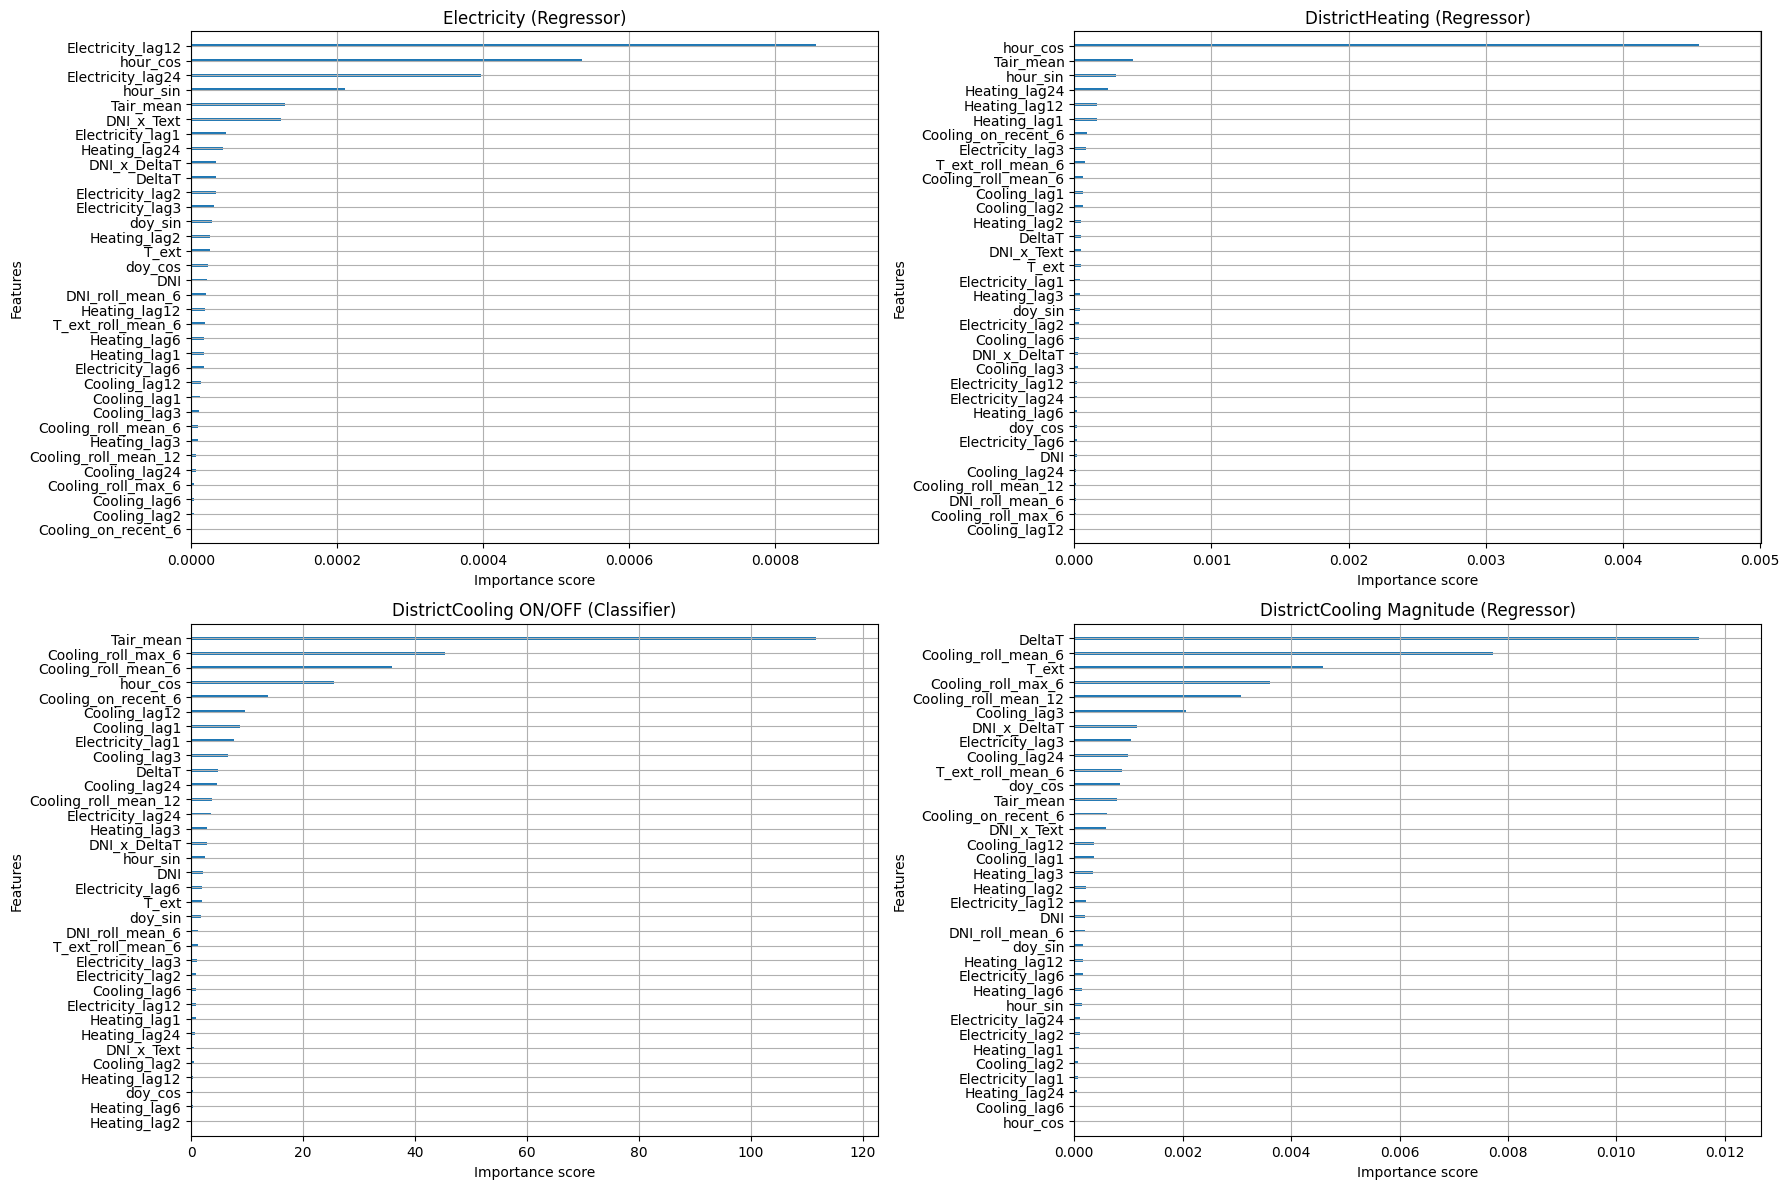
\includegraphics[width=\linewidth]{report_assets/prediction_plot_cell7_out1.png}
    \caption{Feature importance dei 4 modelli interni.}
\end{minipage}\hfill
\begin{minipage}{0.49\linewidth}
    \centering
    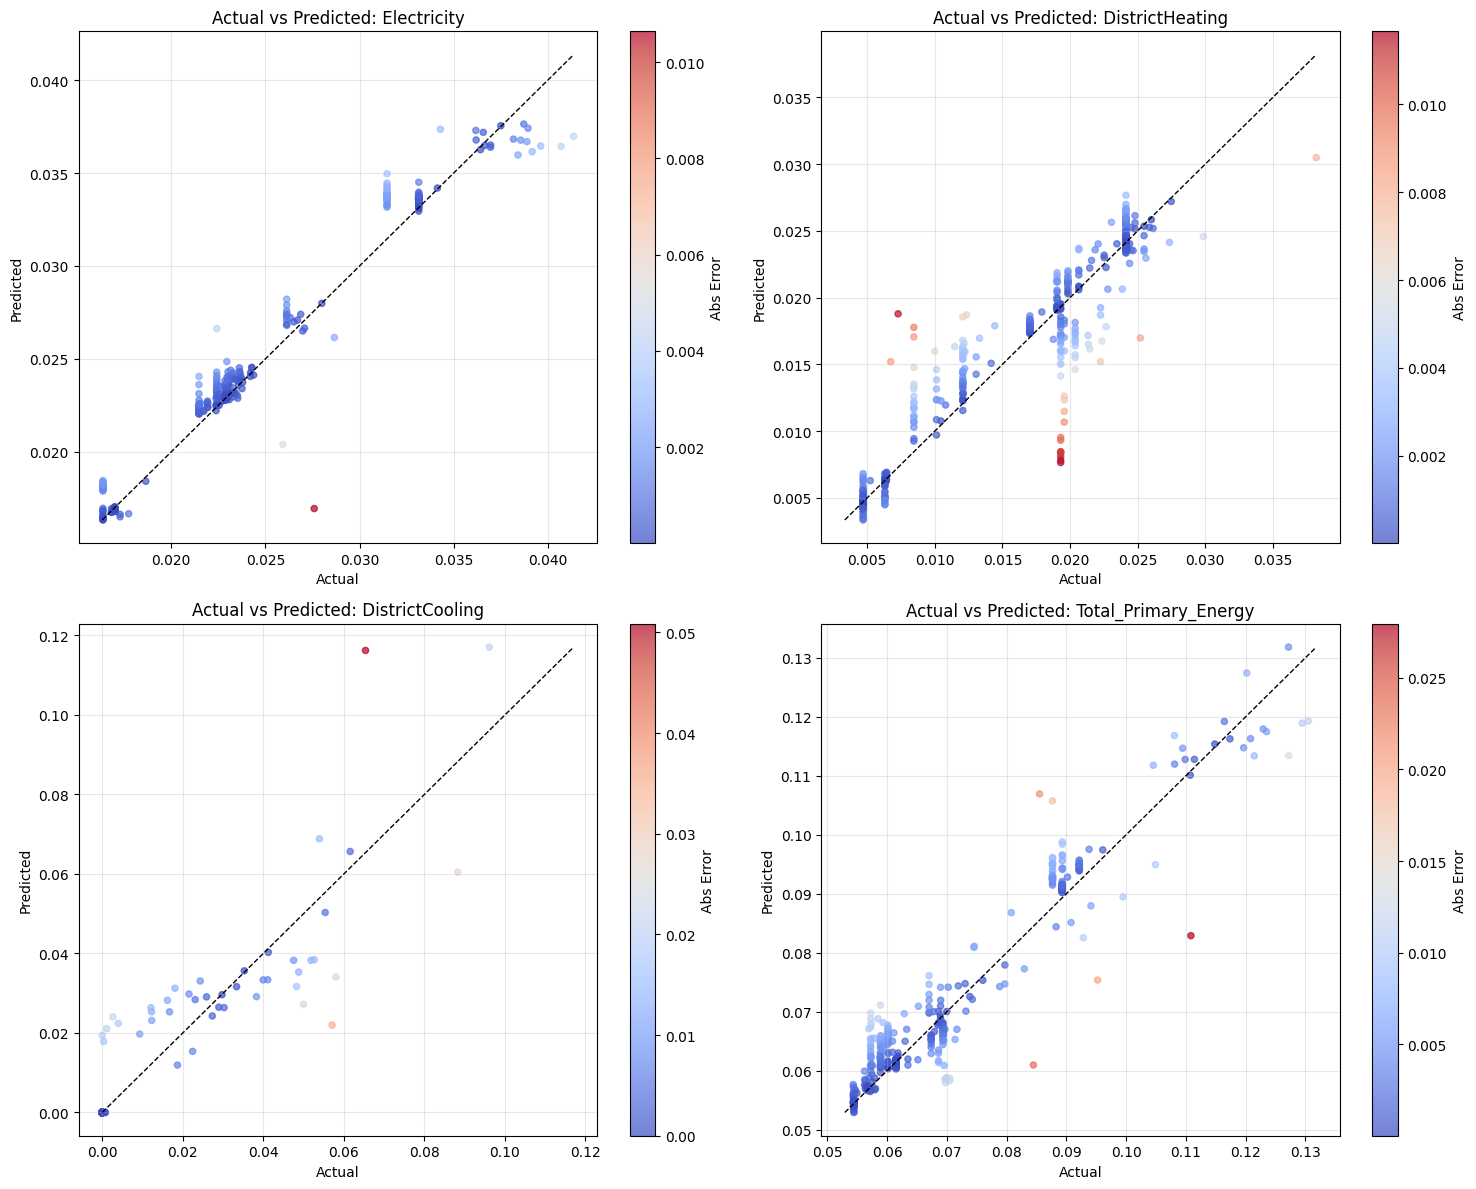
\includegraphics[width=\linewidth]{report_assets/prediction_plot_cell8_out1.png}
    \caption{Predetto vs reale (errore in colore).}
\end{minipage}
\end{figure}

\begin{figure}[H]
\centering
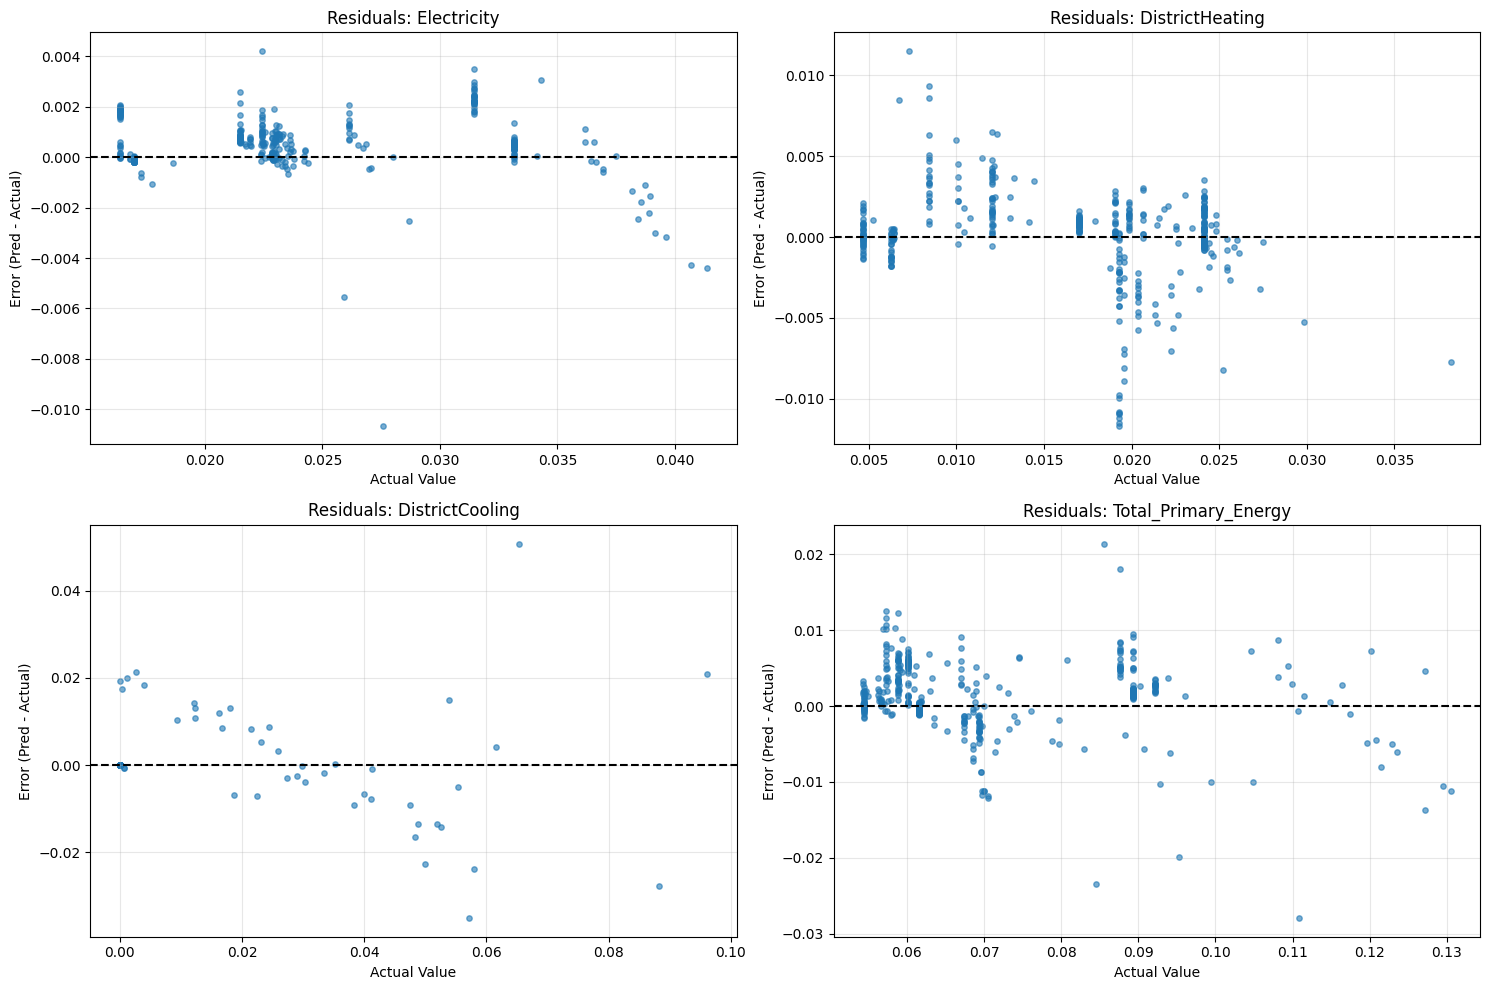
\includegraphics[width=0.76\linewidth]{report_assets/prediction_plot_cell9_out1.png}
\caption{Residui vs valori reali: dispersione più alta alle code, soprattutto sul cooling.}
\end{figure}

\section*{5. Conclusioni operative}
\begin{itemize}
    \item Pipeline \textbf{causale} e \textbf{coerente con la fisica dell'edificio}.
    \item Prestazioni molto alte su Electricity e Total Primary Energy.
    \item Buon comportamento globale su Heating/Cooling; margine di miglioramento sui picchi cooling ON.
    \item Deploy realistico con due accortezze: warm-up iniziale per le lag (prime 24 finestre) e retraining periodico in caso di drift.
\end{itemize}

\vfill
\small
Modello salvato in \texttt{xgb\_flat2\_model.joblib}. Notebook: \texttt{PredictionAlgoithm.ipynb}.

\end{document}
